\section{Localisation}
Mobile robots navigating in accordance to a map, need localisation.
There are various localisation methods and sensors for mobile robots.
This section describes how a localisation method was implemented % on a 'Nexus Robot'
with data from the robot's encoders and its laser range scanner.
Due to time constraints, the method was implemented as an offline program
on a PC, using data gathered by a Nexus Robot, instead of as an online program
running on the Nexus Robot as it moved.
\subsection{Method}
For the localisation part of the project it was chosen to compare two different approaches:

\begin{itemize}
	\item Position estimate based on odometry (wheel encoders).
	\item Position estimate based on line features extracted from the laser range scanner. 
\end{itemize}

Both of these approaches rely on a known starting location.
The second also needs knowledge of the environment
 - it must  compare the extracted features with probable features from the map
(based on last know location of the robot). 


The mobile robot used is a Nexus Robot - 2WD mobile robot kit 10004 (figure \ref{nexus_robot}),
fitted with a laser range scanner of type Hokuyo URG-04LX-LG (figure \ref{laserrange}). 

\begin{figure}[ht]
\centering
  \begin{subfigure}[t]{0.3\textwidth}
    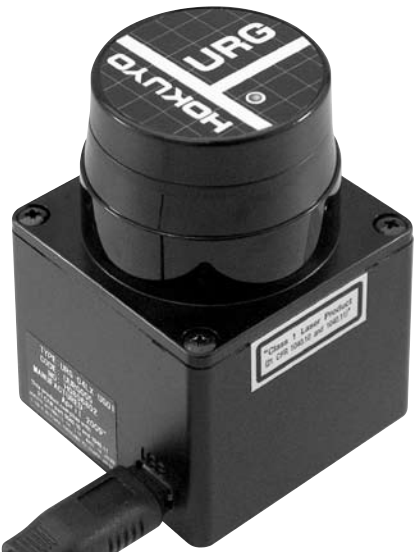
\includegraphics[width = \textwidth]{graphics/hokuyo_laserrange}
    \caption{Hokuyo URG-04LX-LG laser range scanner.}
    \label{laserrange}
  \end{subfigure}
  \begin{subfigure}[t]{0.4\textwidth}
    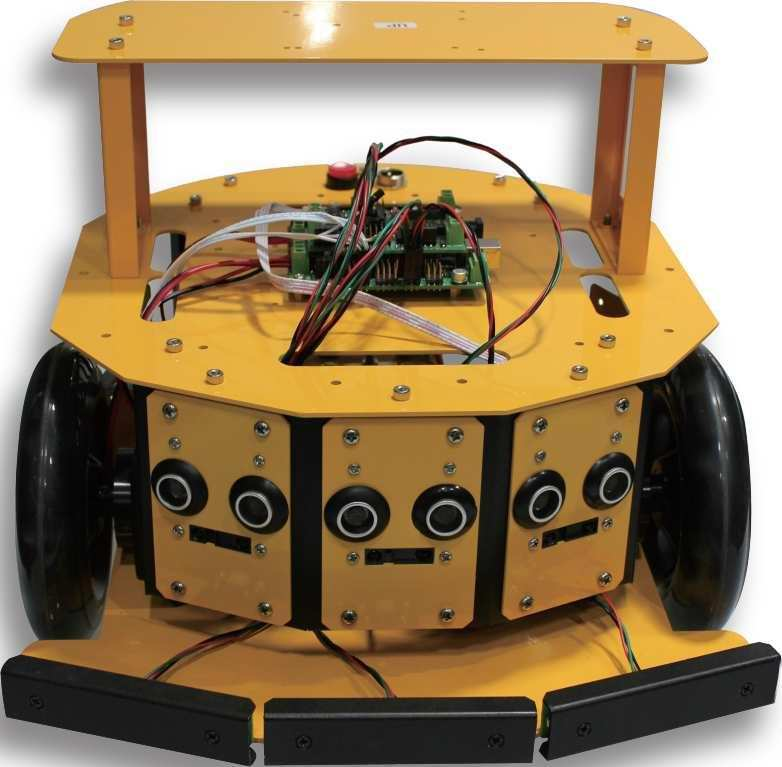
\includegraphics[width = \textwidth]{graphics/nexus_robot}
    \caption{Nexus Robot - 2WD mobile robot kit 10004.}
    \label{nexus_robot}
  \end{subfigure}
    \caption{Hardware used}
\end{figure}

\subsubsection{Gathering data using UMBmark}
The performance of the localisation technique was measured using UMBmark. 
The position before and after following a preprogrammed path through a 1 x 1 [m] square %5 times
was compared for the different localisation techniques.
%The planned path is shown in figure 
%\todo[inline, author=Michael]{I need picture of it here..}
While testing, the robot was not given any feedback from the sensors.
After each $90 \degree$ turn, the robot stopped and its position on the test track was measured for reference.  
Sensor readings from both the encoders and the laser range scanner were gathered and saved for further offline processing. 
This means that 3 different measurements of the position were gathered: 
\begin{itemize}
	\item Reference position (measured with tape).
	\item Position based on encoder feedback. 
	\item Position based on feature extraction using the laser range scanner. 
\end{itemize}

\subsubsection{Position based on odometry}
%\todo[inline, author=Michael]{Based on (or ripped off :P ) sec. 5.2.4 from our lovely friend, siegwart.}
The position/state $Q$ of the robot is represented by the vector: 
\begin{equation}
  Q_r = 
  \begin{bmatrix}
    x_r \\
    y_r \\
    \alpha_r
  \end{bmatrix}
\end{equation}
The robots position is estimated from the previous position, plus the movement in the last time period $\Delta t$.
The change in position $\Delta Q_r$ from each timestep is added to the position.
This can be written as 
\begin{equation}
  Q_r\textrm' = Q_r + \Delta Q_r
\end{equation}
The feedback from the robot is given as the movement of each wheel in millimetres.
$\Delta Q_r$ can be found from the following equations: 
\begin{eqnarray}
	\Delta x_r &=& \Delta s \cos \left(\alpha_r + \frac{\Delta \alpha_r}{2}\right) \\
	\Delta y_r &=& \Delta s \sin \left(\alpha_r + \frac{\Delta \alpha_r}{2}\right) \\
	\Delta \alpha_r &=& \frac{\Delta s_r + \Delta s_l}{b} \\
	\Delta s &=& \frac{\Delta s_r + \Delta s_l}{2} \\
\end{eqnarray}
Where $\Delta s_r and \Delta s_l$ are the distances traveled by the right and the left wheels
and $b$ is the distance between the robots two wheels. Adding this together, the equation for the updated position is: 
\begin{equation}
  Q_r\textrm' = 
  \begin{bmatrix}
    x_r \\
    y_r \\
    \alpha_r
  \end{bmatrix}
  +
  \begin{bmatrix}
    \Delta s \cos \left(\alpha_r + \frac{\Delta \alpha_r}{2}\right) \\
    \Delta s \sin \left(\alpha_r + \frac{\Delta \alpha_r}{2}\right) \\
    \frac{\Delta s_r + \Delta s_l}{b}
  \end{bmatrix}
\end{equation}
%\todo[inline, author=Michael]{Maybe add an interfacing of scanner subsubsection here?}
%\todo[inline, author=Michael]{And so he wrote a section :P}
\subsubsection{Getting data from the laser range scanner}
The Hokuyo laser scanner measures distance to the nearest obstacles in a $240 \degree$ range as shown in figure \ref{fig:laserrange_angle}. The angular resolution is $0.352 \degree$ which gives 681 data points for each scan. The scanning rate is 10 Hz.

\begin{figure}
 \centering
 \begin{tikzpicture}[scale=0.5]
 
 \draw[dashed] (-5,0) node[left] {\(\frac{\pi}{2}\)} -- (5,0) node[right] {\(\frac{3\pi}{2}\)};
 \draw[dashed] (0,-5) -- (0,5) node[above] {\(0\)};
 
 \node[name=robot] at (0,0) {\includegraphics[width=2.5cm]{graphics/robot2}};
 \fill[pattern color=gray!50, pattern=crosshatch]  (robot.center) -- (210:5cm) arc(210:330:5cm);
 \fill[pattern color=red!50,  pattern=crosshatch]  (robot.center) -- (330:5cm) arc(-30:210:5cm);
 
 \end{tikzpicture}
 \caption{The area covered by the laser range scanner.}
 \label{fig:laserrange_angle}
 \end{figure}

The laser range scanner communicates with the computer using Serial over USB. The serial communication uses the SCIP 2.0 serial protocol. 
A basic application for gathering data from the laser range was written
in C++\footnote{The program is called "hokuyo\_laserrange" in the included "code" directory}.
The program gathers and decodes the data received, and saves it as a CSV file.
The program stops the laser range scanner when the UMBmark test is terminated.

%%%%%%%%%%%
\subsection{Feature Detection}
To detect the features of the robots whereabouts it was decided to implement RanSaC. During tests of this implementation it was found that the lines generated in with RanSaC had tendencies to detect two similar lines next to each other for the same features, when his feature was represented by many points in the sample. It was hence decided to implement the RanSaC with a merge function. The angle and distance to the two lines representing the same feature where then averaged to give one line.

%Furthermore a variation of RanSaC was made. This implementation was then compared to the traditional RanSaC method, using the same parameters, on a dataset collected from the 2D laser scanner while performing the UMB mark test (driving in a $ 1 x 1 m$ square). This gave 1761 unique data set samples from the 2D scanner in the dataset used to test.
%The  the lines are plotted in matlab against the data points from the 2D scanner. The number of lines plotted where no features should be found was then counted for the whole data set and compared.


It was decided to represent all lines as polar lines, with $ (theta, rho) $. All lines are, for simplicity, standardized to conform with $ 0 <= theta < 2*PI $ and $ rho >= 0 $. The modified version of RanSaC was implemented as follows:

\begin{enumerate}
\item Copy the data from the 2D laser scanner into a list, $ \Lambda_{points} $ , of polar points $ (theta, rho) $, excluding all points with $ rho = 0 $ which correspond to not-visible points to the scanner.
\item Copy two unique random points into $ \Lambda_{sample} $ and find the line, $ \lambda_{init} $, passing through them. \label{item:genRandomPoints_LamdaInit}
\item Copy all points within $ \Delta_{max deviation} $ distance to $ \lambda_{init} $ into $ \Lambda_{sample} $. If the size of $ \Lambda_{sample} $ passes a minimum threshold, go to item \ref{item:tresholdPassed_RemovePoints} else go to \ref{item:genRandomPoints_LamdaInit}.
\item Delete all points from $ \Lambda_{points} $) within $ \Delta_{max deviation} $ from $ \lambda_{init} $.\label{item:tresholdPassed_RemovePoints}
\item Find the best fit line, $ \lambda_{final} $ , passing through the dataset $ \Lambda_{sample} $. $ \lambda_{final} $ in the final line set.
\item Until a specific number of RanSaC-loops done without finding a line or dataset too small to contain a valid line go to item \ref{item:genRandomPoints_LamdaInit} else continue.
\item Standardize the lines found to fit the specified format and merge lines considered to represent the same feature.
%\item Recompute the line for $ \Lambda_{final} $ and store the line. Go then to item \ref{item:genRandomPoints_LamdaInit}.
%\item Move all data points back to $ \Lambda_{points} $ and go back to \ref{item:genRandomPoints_LamdaInit}. \label{item:lineNotImproved_refillLamdaPoints}
\end{enumerate}

The data-points form the laser range scanner which where found to be 0 ($ rho = 0 $) are removed because those are, defined by the scanner, points for which the object is out of reach. The parameters for the RanSaC where experimentally found to fit the robots data points collected as best as possible.


%%%%%%%%%%%%

\subsubsection{Position based on features from laser range scanner}
The state of the robot is in polar coordinates represented  as 
$$Q_r = \begin{pmatrix}
R_r\\
\theta_r\\
\alpha_r
\end{pmatrix}$$ 
and in cartesian coordinates as 
$$Q_r = \begin{pmatrix}
x_r\\
y_r\\
\alpha_r
\end{pmatrix}$$

When the localisation program starts, it has a map of the room the robot is in.
The map consists four walls, each represented as 
$$wall_n = \begin{pmatrix}
R_n\\
\theta_n
\end{pmatrix}
$$

The initial position of the robot is also known on startup.

The localisation algorithm is illustrated as a flowchart in figure \ref{fig:localisation}.
An illustration of the global coordinate system and the robot's coordinate system can be seen 
in figure \ref{fig:coord}.

\paragraph*{Mapping}
The found lines are all represented in the robot's coordinate system, relative to the robot position and orientation.
These lines are mapped into the global coordinate system, using the last known robot state. Using 
the last known state of the robot to map the lines will give some mapping-error.
The found lines are then compared to the map. If a found line matches a line 
in the map, within a certain threshold, it is concluded, that they are in 
reality the same line and that the difference is due to the mapping error.

\paragraph*{Updating robot state}
There are several scenarios of what the program will do after the matching of lines,
depending on the lines that have been matched.
The philosophy of the algorithm is that the lines should be used as much as possible,
to determine the robot state.

If no lines have been matched, the robot state remains the same, and is not updated.

If only one line has been matched, the robot orientation \(\alpha_r\) will be updated
so that the found line aligns with the known line in the global map.
The same strategy is used if there are several matched lines, and the new \(\alpha_r\) is
found by averaging the individual orientations.

If two intersecting lines have been matched (and a corner found), the robots position is constrained to
an intersection between two lines. Again, finding the intersection is a matter of moving the global
lines towards the origin by the distance from the robot to the walls,
and then finding the intersection between the two lines.
If more than two intersecting lines are matched, the same strategy is used and the new position
is calculated as the average of all the found positions.

Thus, as long as at least one line is matched, the robot state is updated.
The update correctness should improve with the number of lines matched,
especially if the lines are not parallel.

The weakness of the algorithm lies in missed data points, or data points with no lines detected by RanSaC.
The further the robot actually moves from the last updated position, the harder it is to match the line
feature to the global map, and eventually the lines would be matched incorrectly.

\begin{figure}
  \centering
    \tikzstyle{node} = [rectangle, rounded corners, minimum width=3cm, minimum height=1cm,text width = 4 cm,text centered, draw=black, fill=red!30]
    \tikzstyle{io} = [trapezium, trapezium left angle=70, trapezium right angle=110, text width = 4cm,minimum width=1cm,minimum height=1cm, text centered, draw=black, fill=blue!30]
    \tikzstyle{io1} = [trapezium, trapezium left angle=70, trapezium right angle=110, minimum width=1cm,minimum height=1cm, text centered, draw=black, fill=blue!30]
    \tikzstyle{process} = [rectangle, minimum width=3cm, minimum height=1cm,text width = 4cm,text centered, draw=black, fill=orange!30]
    \tikzstyle{decision} = [diamond, minimum width=3cm, minimum height=1cm,text width = 2cm,text centered, draw=black, fill=green!30]    
    \tikzstyle{arrow} = [thick,->,>=stealth]

\begin{tikzpicture}[node distance=2.2cm,scale=0.8, every node/.style={scale=0.8}]

%% NODES
\node (start) [node] {Robot is booted.  State is known};
\node (input) [io, below of=start] { Input from laser range scanner };
\node (input1) [io1, left of=input, xshift=-2.5cm] {10 Hz };
\node (pro1) [process, below of=input] {Line extraction algorihthm on laser range data};
\node (pro2) [process, below of=pro1] {Map the found lines into global map using last robot state};
\node (dec1) [decision, below of =pro2, yshift=-1.2cm] {Number of found lines};
\node (pro4) [node, left of=dec1, xshift = -3cm ] {Do not update robot state};
\node (pro5) [process, below of=dec1, yshift = -1cm ] {Calculate robot orientation from found line(s)};
\node (pro6) [node, below of=pro5,yshift =-0.5cm] {Update robot state};
\node (dec2) [decision,right of= dec1, xshift =2cm] {Number of corners};
\node (pro3) [process, right of =dec2, xshift = 2.5cm ] {Calculate full robot state from found lines};



%% ARROWS
\draw [arrow] (start) -- (input);
\draw [arrow] (input) -- (pro1);
\draw [arrow] (pro1) -- (pro2);
\draw [arrow] (pro2) -- (dec1);
\draw [arrow] (dec1) -- node[anchor=south] {$\geq$1} (dec2);
\draw [arrow] (dec1) -- node[anchor=south] {0} (pro4);
%\draw [arrow] (dec1) -- node[anchor=east] {1} (pro5);
\draw [arrow] (pro5) -- (pro6);
\draw [arrow] (pro3) |- (pro6);
\draw [arrow] (input1) -- (input);
\draw [arrow] (dec2) |- node[anchor=north] {0}(pro5);
\draw [arrow] (dec2) -- node[anchor=south] {$\geq$1} (pro3);
\end{tikzpicture}
    \caption{The localisation method, purely based on data from laser range scanner.}
  \label{fig:localisation}
\end{figure}


\begin{figure}
  \centering
\begin{tikzpicture}[scale=2]
%set angles here. wall angle is what laser range scanner measures  (relative to robot)
\newcommand{\robotAngle}{30}
\newcommand{\wallAngle}{20}

                                                                                                                             %coordinate axis
\draw[->] (0,0) -- (5,0) node[right]                                                                                         {\(x_{global}\)};
\draw[->] (0,0) -- (0,5) node[above]                                                                                         {\(y_{global}\)};

%robot
\node[name=robot] at (\robotAngle:2cm) {};

                                                                                                                             %robot relative coordinate axis
\draw[rotate=\robotAngle,->] (robot.center) -- ++(3,0) node[right]                                                           {\(x_{robot}\)};
\draw[rotate=\robotAngle,->] (robot.center) -- ++(0,3) node[right]                                                           {\(y_{robot}\)};

%calculate theta_2
\FPeval{\thetaTwo}{clip(\robotAngle + \wallAngle)}        

%wall
\node[scale=0.3,fill=black, minimum width=15cm, rotate={90 + \robotAngle + \wallAngle}, name=wall] at ([shift=(\thetaTwo:2cm)] robot.center) {};
\node[name=midwall] at ($(wall.180)!(robot.center)!(wall.0)$) {};
\node[above] at (wall.0) {wall};

                                                                                                                             %laser range output
\draw[very thick, red]  (midwall.center) -- (robot.center) node[black,midway, left]                                          {\(r\)};
\draw[very thick, red]   ([shift=(\robotAngle:1cm)] robot.center) arc(\robotAngle:\thetaTwo:1cm) node[near end, black,right] {\(\theta_{wall}\)};

                                                                                                                             %robot position
\draw[dashed] (robot.center) -- ++(3,0) node[right]                                                                          {\tiny\( 0\degree\)};
\draw[dashed] (robot.center) -- ++(0,3) node[above]                                                                          {\tiny\(\frac{\pi}{2}\degree\)};
\draw[very thick, green] ([shift=(\robotAngle:1cm)] robot.center) arc(\robotAngle:0:1cm)  node[midway, black,right]          {\(\alpha\)};

                                                                                                                             %summated vector of robot and wall angle
\path (midwall); \pgfgetlastxy{\XCoord}{\YCoord};
\draw[very thick, dashed, green] (0,0) -- (midwall) node[black, midway, left]                                                {\(r_1\)};
\draw[very thick, green] (0.5,0) arc(0:{atan(\YCoord/\XCoord)}:0.5cm) node[midway, black, right]                             {\(\theta\)};
                                                                                                                             
                                                                                                                             %real angle to wall                                                                                                          
\node[name=projected] at ($(wall.180)!(0,0)!(wall.0)$) {};                                                                   
\draw[very thick, dashed,blue] (projected.center) -- (0,0) node[black, midway, left]                                         {\(r_2\)};
\draw[very thick, blue] (1.5,0) arc(0:\thetaTwo:1.5cm) node[midway, black,right]                                             {\(\theta_2\)};

                                                                                                                             %I am not sure what we use this angle for...
\draw[dashed,red!50] (0,0) -- (robot.center) ;
\draw[very thick,red!50] ([shift=(\robotAngle:1cm)] (0,0) arc(\robotAngle:0:1cm) node[midway,black,right]                    {\(\theta_1\)};

\end{tikzpicture}
 \caption{Illustration of the global coordinate system and the robot's coordinate system}
  \label{fig:coord}
\end{figure}
